%        File: ucore_thumips.tex
%     Created: Fri Apr 06 12:00 PM 2012 C
% Last Change: Fri Apr 06 12:00 PM 2012 C
%
\documentclass[a4paper]{article}
\usepackage{graphicx}
\usepackage{indentfirst}
\usepackage{algorithm}
\usepackage{xcolor}
\usepackage{listings}

\definecolor{dkgreen}{rgb}{0,0.6,0}
\definecolor{gray}{rgb}{0.5,0.5,0.5}
\definecolor{mauve}{rgb}{0.58,0,0.82}

\lstset{ %
  basicstyle=\footnotesize,           % the size of the fonts that are used for the code
  numbers=none,                   % where to put the line-numbers
  numberstyle=\footnotesize,          % the size of the fonts that are used for the line-numbers
  stepnumber=2,                   % the step between two line-numbers. If it's 1, each line
                                  % will be numbered
  numbersep=5pt,                  % how far the line-numbers are from the code
  backgroundcolor=\color{white},      % choose the background color. You must add \usepackage{color}
  showspaces=false,               % show spaces adding particular underscores
  showstringspaces=false,         % underline spaces within strings
  showtabs=false,                 % show tabs within strings adding particular underscores
  frame=none,                   % adds a frame around the code
  tabsize=2,                      % sets default tabsize to 2 spaces
  captionpos=b,                   % sets the caption-position to bottom
  breaklines=true,                % sets automatic line breaking
  breakatwhitespace=false,        % sets if automatic breaks should only happen at whitespace
  title=\lstname,                   % show the filename of files included with \lstinputlisting;
                                  % also try caption instead of title
  numberstyle=\tiny\color{gray},        % line number style
  keywordstyle=\color{blue},          % keyword style
  commentstyle=\color{dkgreen},       % comment style
  stringstyle=\color{mauve},         % string literal style
  escapeinside={\%*}{*)},            % if you want to add a comment within your code
  morekeywords={*,...}               % if you want to add more keywords to the set
}


\begin{document}
\title{UCORE Porting on MIPS32S CPU}
\author{Chen Yuheng\\ Tsinghua Unv.}
\maketitle

\section{Introduction}
This report gives a brief introduction to our project -- 
\emph{UCORE} porting onto the MIPS32S platform, including the kernel, limited
device drivers as well as the user-lib. \emph{UCORE} is an experimental 
modern operating system that includes a basic memory manager, a limited process/
thread scheduler, linux-like VFS and incomplete POSIX-compatible syscall 
interface.  Currently, the following platforms are supported:
 \begin{itemize}
   \item \emph{Mipssim in Qemu}, which is simulated with qemu-system-mipsel.
     The hardware configuration is available in qemu's source code,
     several important components of which is summarized in
     Table. \ref{tab:mipssim}.
     \begin{table}[h]
       \centering
       \begin{tabular}{|r|rrr|}
         \hline
         Component & Type & Base Address &  IRQ \\
         \hline
         Uart & 16450 & 0x1fd003f8 & 4 \\
         Timer & On Chip & -- & 7 \\
         PIC   & On Chip & -- & -- \\
         \hline
       \end{tabular}
       \caption{Mipssim Hardware Configuration}
       \label{tab:mipssim}
     \end{table}

   \item \emph{Our FPGA MIPS32S Implementation} hardware platform.
 \end{itemize}

Our code is available on Github
\footnote{https://github.com/chyh1990/ucore-thumips}
 and is kept updating. Any bug reports are welcomed.

\section{Architecture of the MIPS32S Platform}

\section{Development Environment}
This section is a guide to setup and use the cross-compile development environment for Mips.

\subsection{Toolchain}
We use the standard toolchain GCC for Mips to compile ucore, even on our 
MIPS32S CPU, in which only a subset of MIPS1 Instruction Set is implemented.
The best place to get a free GCC-MIPS toolchain is on CodeSourcery
\footnote{https://sourcery.mentor.com/GNUToolchain/release2189}, just make sure you download GCC 4.6. The package also includes gdb for MIPS.

Another way to get a toolchain is compiling it from source code. GCC-core 4.6.3+Binutils 2.22 is tested. Compiling GCC is tricky, just google it if you
come into any issues. Here is my configuration for GCC on 64-bit Ubuntu 12.04:

\begin{verbatim}
../gcc-4.6.3/configure --prefix=/home/guest/cpu/build-gcc/mips_gcc 
  --target=mips-sde-elf --disable-nls --enable-languages=c  
  --disable-multilib --without-headers --disable-shared
  --without-newlib --disable-libgomp -disable-libssp 
  --disable-threads --disable-libgcc
\end{verbatim}


\subsection{Simulator}
You can run ucore-thumips with the standard Qemu in your Linux distribution:

\begin{verbatim}
qemu-system-mipsel -M mipssim -m 32M -serial stdio 
  -kernel obj/ucore-kernel-initrd
\end{verbatim}

But we recommend to use our modified Qemu to simulate our simplified MIPS Instruction Set
and Flash support. 

what's more, it will be necessary to setup the mips-sde-elf-gdb properly, refer to 
the following \emph{.gdbinit} example:

\begin{verbatim}
set endian little
set mipsfpu none
target remote 127.0.0.1:1234
file obj/ucore-kernel-initrd
\end{verbatim}


\subsection{MIPS32S Programming Guide}
MIPS32S supports a simpified MIPS32 Intruction Set, here is several important differences:

\begin{enumerate}
\item No \emph{lh/sh}
\item No \emph{divu}
\item No \emph{add/sub}, only \emph{addu/subu} is supported.
\end{enumerate}

We use some tricks to solve these problems, see \emph{kern/thumips.h}.

Another problem is that MIPS32S does NOT support delayed slot. Solving 
this problem by giving GCC options correctly:

\begin{verbatim}
CFLAGS	:=  -EL -G0 -fno-delayed-branch -Wa,-O0
\end{verbatim}

An example MIPS32S C project can be found in test1.tar.gz.


\section{Source Code Organization}
This section introduces the source code orginazation of ucore-thumips
and explains several configuration options.
\subsection{Source Tree}
Since our work is based on LAB0-LAB8, important directories are listed in Table. \ref{tab:dir}.

\begin{table}[h]
  \centering
  \begin{tabular}{|l|l|}
    \hline
    Directory & Description \\
    \hline
    debug  &     debug console after a kernel panic \\
    driver &     device driver interface definition \\
    include &    useful macros for MIPS32S \\
    fs     &     Filesystem \\
    init   &     kernel entry point and initialization code \\
    libs   &     utilities \\
    mm     &     low-level memory management \\
    process   &  context switch             \\
    sync   &     atomic operation           \\
    syscall &     MIPS-specific syscall machanism \\
    trap   &     exception handling  \\
    \hline
  \end{tabular}
  \caption{ucore-thumpis directories}
  \label{tab:dir}
\end{table}

\subsection{Makefile}
UCore does not have a configuration system yet, all configuration
is hand-coded in the Makefile.
\begin{enumerate}
\item \emph{GCCPREFIX}, toolchain path;
\item \emph{USER\_APPLIST}, the applications to be included.
\end{enumerate}

More detailed memory layout is defined in memlayout.h in the corresponding
machine directory, see Section. \ref{sec:mm}.

\section{Implementation Details}
This section describes the implementations of some important mechanism 
in the MIPS32S CPU, which is similar to the standard MIPS32 CPU.
Thus, I refer to Harvard's OS/161\cite{OS161} project during writing the code.

\subsection{Booting}
The booting process is also simulated. Our Qemu needs the following files:

\begin{table}[h]
\centering
\begin{tabular}{|l|l|l|}
\hline
 File & Type & Description \\
\hline
ucore-kernel-initrd & ELF & ucore kernel with ramdisk\\
flash.img & Binary & used for flash simulation, can be a link to the kernel\\
boot/loader.bin & Binary & BIOS, knows ELF and load kernel from Flash\\
thumips\_insn.txt & Text & Instruction Set Descriptor\\
\hline
\end{tabular}
\caption{Qemu Files}
\label{tab:qemufile}
\end{table}


There is two ways to use our modified Qemu
to boot ucoer for MIPS. 

\begin{table}[h]
  \centering
  \begin{tabular}{|r|r|r|}
    \hline
    Offset & Size & Usage\\
    \hline
    0x00000000 & 0x80000000 & Userspace, TLB mapped\\
    0x80000000 & 0x20000000 & Kernel Space, Direct mapping \\
    0xA0000000 & 0x20000000 & IO Space, Direct Mapping \\
    \hline
  \end{tabular}
  \caption{Bootable Kernel Memory Layout}
  \label{tab:layout}
\end{table}

Then, the C enironment must be setup:
\begin{itemize}
\item \emph{sp}, setup the stack
\item \emph{gp}, set to \_gp (defined in ldscript)
\item zero .bss section
\end{itemize}

For convenience, root filesystem image(ramdisk) is linked
with the kernel, appending at the end of the \emph{.data} section.
\footnote{see tools/kernel.ld}.

\subsection{Exception Handling}
The most important hardware support for exception/interrupt handling on MIPS32S is the \emph{SR}
register:

\begin{figure}[h]
\centering
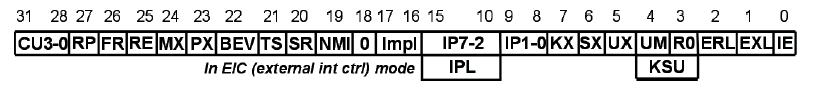
\includegraphics[width=0.8\linewidth]{reg-sr.png}
\caption{Status Register\cite{Sweetman:2006:SMR:1210986}}
\label{fig:reg-sr}
\end{figure}

\begin{itemize}
\item ERL, MUST be clear by software after reset;
\item EXL and KSU, MUST be set properly to handle nested exceptions.
\end{itemize}

The kernel use a trapframe structure to save registers when privilege mode transition occurs:
\begin{algorithm}[h]
   \begin{lstlisting}[language={C++}]
/* $1 - $30 */
struct pushregs {
 uint32_t reg_r[30];
};

/*
 * Structure describing what is saved on the stack during entry to
 * the exception handler.
 *
 * This must agree with the code in exception.S.
 */

struct trapframe {
	uint32_t tf_vaddr;	/* coprocessor 0 vaddr register */
	uint32_t tf_status;	/* coprocessor 0 status register */
	uint32_t tf_cause;	/* coprocessor 0 cause register */
	uint32_t tf_lo;
	uint32_t tf_hi;
	uint32_t tf_ra;	/* Saved register 31 */
  struct pushregs tf_regs;
	uint32_t tf_epc;	/* coprocessor 0 epc register */
};

\end{lstlisting}
\caption{Trapframe}
\end{algorithm}

The trapframe is constructed by the assembly in trap/exception.S, be aware with the fact that
registers \emph{k0} and \emph{k1} is reserved by the compiler so we can use them in the exception
handler without saving them.

See \emph{kern/trap/exception.S} for more details.

\subsection{Memory Management}
\label{sec:mm}
MIPS32S has no MMUs, but has a programmable TLB unit. So
it is possible to emulate MMU utilizing the TLB miss exception.
The software simulated MMU of MIPS32S is similar to X86's, 
Ucore uses the following 
configuration (which is similar to X86's VA layout) :

\begin{table}[H]
\centering
\begin{tabular}{|c|c|c|}
\hline
PDT Index & PTE Index & Offset \\
\hline
10 & 10 & 12 \\
\hline
\end{tabular}
\caption{Virtual Address in ucore}
\label{tab:va_layout}
\end{table}

In our TLB miss handler, we first checkout whether it is just a TLB miss
or a page table miss by looking the address up in our emulated X86 page table.
If it is a TLB miss, check the access permission and fill it up (or raise a
access violation). If it is a page miss, call the do\_pgfault. See Alg. \ref{alg:tlbmiss}.


\begin{algorithm}[h]

 \begin{lstlisting}[language={C++}]

/* use software emulated X86 pgfault */
static void handle_tlbmiss(struct trapframe* tf, int write)
{
  int in_kernel = trap_in_kernel(tf);
  assert(current_pgdir != NULL);
  uint32_t badaddr = tf->tf_vaddr;
  int ret = 0;
  pte_t *pte = get_pte(current_pgdir, tf->tf_vaddr, 0);
  if(pte==NULL || ptep_invalid(pte)){   //PTE miss, pgfault
    //tlb will not be refill in do_pgfault,
    //so a vmm pgfault will trigger 2 exception
    //permission check in tlb miss
    ret = pgfault_handler(tf, badaddr, get_error_code(write, pte));
  }else{ //tlb miss only, reload it
    /* refill two slot */
    /* check permission */
    if(in_kernel){
      tlb_refill(badaddr, pte); 
      return;
    }else{
      if(!ptep_u_read(pte)){
        ret = -1;
        goto exit;
      }
      if(write && !ptep_u_write(pte)){
        ret = -2;
        goto exit;
      }
      tlb_refill(badaddr, pte);
      return ;
    }
  }

exit:
  if(ret){
    print_trapframe(tf);
    if(in_kernel){
      panic("unhandled pgfault");
    }else{
      do_exit(-E_KILLED);
    }
  }
  return ;
}

\end{lstlisting}
\caption{User Mode System Calling Convetion}
\label{alg:tlbmiss}
\end{algorithm}

\subsection{Context Switch}
According to MIPS32 O32 ABI, we must save the following registers
during the context switching:

\begin{algorithm}[H]
 \begin{lstlisting}[language={C++}]
struct context {
	uint32_t sf_s0;
	uint32_t sf_s1;
	uint32_t sf_s2;
	uint32_t sf_s3;
	uint32_t sf_s4;
	uint32_t sf_s5;
	uint32_t sf_s6;
	uint32_t sf_s7;
	uint32_t sf_s8;
	uint32_t sf_gp;
	uint32_t sf_ra;
  uint32_t sf_sp;
};

\end{lstlisting}
\caption{Context}
\label{alg:context}
\end{algorithm}

According to O32 ABI, \emph{s0-s8} must be reserved by the callee,
\emph{gp} is a global pointer, \emph{ra} is the interrupted PC.
In addition, we must switch the kernel stack, which is saved in \emph{sf\_sp}.


\subsection{System Call}
The syscall mechanism is borrowed from Linux2.6. In MIPS, a special 
instruction \emph{syscall} handles user mode to supervisor mode transition.

In ucore, we employ the following system calling convention:
\begin{enumerate}
  \item \emph{a0 - a3}, arguments(from left to right)
  \item \emph{v0}, syscall number
  \item \emph{syscall}
  \item return value in \emph{v0}
\end{enumerate}

Syscall is wrapped in user mode library and can be called as a normal 
C function. 

\subsection{User Library and Application}
The code in \emph{user}
should works without modification. However, since \emph{libs-user-ucore/syscall.c} is not compatible with MIPS's 
system calling convetion, we use some macros from Linux
to create our own system call entries. See Alg. \ref{alg:syscall}.

\begin{algorithm}[h]
 \begin{lstlisting}[language={C++}]
static inline int
syscall(int num, ...) {
    va_list ap;
    va_start(ap, num);
    uint32_t arg[MAX_ARGS];
    int i, ret;
    for (i = 0; i < MAX_ARGS; i ++) {
        arg[i] = va_arg(ap, uint32_t);
    }
    va_end(ap);

    num += SYSCALL_BASE;

    asm volatile(
      ".set noreorder;\n"
      "move $v0, %1;\n" /* syscall no. */
      "move $a0, %2;\n"
      "move $a1, %3;\n"
      "move $a2, %4;\n"
      "move $a3, %5;\n"
      "syscall;\n"
      "nop;\n"
      "move %0, $v0;\n"
      : "=r"(ret)
      : "r"(num), "r"(arg[0]), "r"(arg[1]), "r"(arg[2]), "r"(arg[3]) 
      : "a0", "a1", "a2", "a3", "v0"
    );
    return ret;
}

\end{lstlisting}
\caption{User Mode System Calling Convetion}
\label{alg:syscall}
\end{algorithm}

Another modification is \emph{user/libs/user.ld}.
The .text section of user application is located at  0x10000000.


\section{Conclusion}
In our project, we work out a basically working version of ucore for MIPS32S.
However, just as what items listed on the TODO list imply,
much work remains for making ucore for MIPS32S pratically usable
operating system.



\bibliographystyle{plain}
\bibliography{book}
\end{document}


